\documentclass[10pt]{article}

\usepackage[margin=0.82in]{geometry}
\usepackage{amsmath,amssymb}
\usepackage{booktabs}
\usepackage{graphicx}
\usepackage{microtype}
\usepackage[numbers,sort&compress]{natbib}
\usepackage[hidelinks]{hyperref}
\usepackage{xcolor}
\usepackage{enumitem}

% Generated from evidence/pilots/*.json; do not hand edit.
\newcommand{\PilotQwenMatrixPass}{5}
\newcommand{\PilotMistralMatrixPass}{5}
\newcommand{\PilotPhiComputePass}{4}
\newcommand{\PilotQwenRatioMin}{0.987}
\newcommand{\PilotQwenRatioMax}{1.007}
\newcommand{\PilotMistralRatioMin}{0.873}
\newcommand{\PilotMistralRatioMax}{1.031}
\newcommand{\PilotAnchorRatio}{1.001}
\newcommand{\PilotAnchorAccuracy}{100\%}
\newcommand{\PilotCheckpointMax}{0.0020}
\newcommand{\PilotAnchorCheckpointGap}{506$\times$}
\newcommand{\PilotCityTwoHopRatio}{0.999}
\newcommand{\PilotCityTwoHopAccuracy}{90\%}
\newcommand{\PilotOtherShift}{0.000}
\newcommand{\PilotVerbalHistoryNoV}{1.004}
\newcommand{\PilotVerbalHistoryV}{0.217}
\newcommand{\PilotVerbalBoth}{0.997}
\newcommand{\ConfirmQwenMatrixPass}{15}
\newcommand{\ConfirmMistralMatrixPass}{15}
\newcommand{\ConfirmQwenRatioMin}{0.985}
\newcommand{\ConfirmQwenRatioMax}{1.010}
\newcommand{\ConfirmMistralRatioMin}{0.939}
\newcommand{\ConfirmMistralRatioMax}{1.004}
\newcommand{\ConfirmQwenAnchorN}{30}
\newcommand{\ConfirmQwenAnchorBelief}{1.075}
\newcommand{\ConfirmQwenAnchorBeliefCI}{[1.068, 1.083]}
\newcommand{\ConfirmQwenAnchorTell}{1.052}
\newcommand{\ConfirmQwenInvariantMin}{70\%}
\newcommand{\ConfirmQwenCheckpointMax}{0.0129}
\newcommand{\ConfirmQwenReadoutMax}{0.877}
\newcommand{\ConfirmMistralAnchorN}{18}
\newcommand{\ConfirmMistralAnchorBelief}{1.076}
\newcommand{\ConfirmMistralAnchorBeliefCI}{[1.062, 1.091]}
\newcommand{\ConfirmMistralAnchorTell}{1.038}
\newcommand{\ConfirmMistralCheckpointMax}{0.0051}
\newcommand{\ConfirmMistralReadoutMax}{0.950}
\newcommand{\ConfirmQwenFourteenAnchorN}{30}
\newcommand{\ConfirmQwenFourteenAnchorBelief}{1.001}
\newcommand{\ConfirmQwenFourteenAnchorBeliefCI}{[1.000, 1.002]}
\newcommand{\ConfirmQwenFourteenAnchorTell}{0.993}
\newcommand{\ConfirmQwenFourteenCheckpointMax}{0.0003}
\newcommand{\ConfirmQwenFourteenReadoutMax}{0.999}
\newcommand{\ConfirmQwenFourteenProbeCheckpointLedger}{100\%}
\newcommand{\ConfirmQwenFourteenProbeCheckpointNarrative}{100\%}
\newcommand{\ConfirmQwenFourteenProbeCheckpointCross}{16.7--18.8\%}
\newcommand{\ConfirmReverseHistory}{0.669}
\newcommand{\ConfirmReverseVerbal}{0.781}
\newcommand{\ConfirmReverseBoth}{1.000}
\newcommand{\ConfirmReverseVerdict}{PARIS\_PRIOR\_REPLICATES\_REVERSE\_BASE}
\newcommand{\ConfirmDeepseekMatrixPass}{12}
\newcommand{\ConfirmDeepseekMatrixEligible}{12}
\newcommand{\ConfirmDeepseekRatioMin}{0.936}
\newcommand{\ConfirmDeepseekRatioMax}{0.977}
\newcommand{\ConfirmDeepseekAnchorBelief}{1.055}
\newcommand{\ConfirmDeepseekAnchorBeliefCI}{[1.034, 1.076]}
\newcommand{\ConfirmDeepseekAnchorTell}{1.013}
\newcommand{\ConfirmDeepseekInvariantBeliefBC}{0\%}
\newcommand{\ConfirmDeepseekCheckpointMax}{0.0054}
\newcommand{\ConfirmDeepseekReadoutMax}{0.953}
\newcommand{\ConfirmGemmaMatrixPass}{15}
\newcommand{\ConfirmGemmaRatioMin}{0.982}
\newcommand{\ConfirmGemmaRatioMax}{1.000}
\newcommand{\ConfirmGemmaCityTwoHopMin}{0.992}
\newcommand{\ConfirmGemmaCityTwoHopMax}{1.007}
\newcommand{\ConfirmGemmaAnchorBelief}{1.073}
\newcommand{\ConfirmGemmaAnchorBeliefCI}{[1.066, 1.081]}
\newcommand{\ConfirmGemmaAnchorTell}{1.013}
\newcommand{\ConfirmGemmaCheckpointMax}{0.0024}
\newcommand{\ConfirmGemmaReadoutMax}{0.936}
\newcommand{\ConfirmLocusLastSufficientLayer}{32}
\newcommand{\ConfirmLocusSourceForwardMin}{0.999}
\newcommand{\ConfirmLocusSourceForwardMax}{1.012}
\newcommand{\ConfirmLocusSourceReverseMin}{0.962}
\newcommand{\ConfirmLocusSourceReverseMax}{1.005}
\newcommand{\ConfirmLocusMarkerMax}{0.0003}
\newcommand{\ConfirmLocusSummaryMax}{0.0005}
\newcommand{\ConfirmLocusNoAcMax}{0.031}
\newcommand{\ConfirmLocusRandomMax}{0.0032}
\newcommand{\ConfirmLocusLThirtySix}{0.402}
\newcommand{\ConfirmLocusLFortyOne}{0.245}
\newcommand{\ConfirmLocusLFortySix}{0.001}
\newcommand{\ConfirmAnchorP}{0.01}
\newcommand{\ConfirmQwenCityTwoHopMin}{0.974}
\newcommand{\ConfirmQwenCityTwoHopMax}{1.002}
\newcommand{\ConfirmQwenCityTwoHopAccMin}{96.7\%}
\newcommand{\ConfirmQwenSpecificityPass}{2}
\newcommand{\ConfirmQwenSpecificityIneligible}{1}
\newcommand{\ConfirmCloseoutVerdict}{PAPER1\_CLOSEOUT\_BOUNDARY}
\newcommand{\ConfirmCloseoutExactLastLayer}{32}
\newcommand{\ConfirmNaturalAnchorBelief}{1.012}
\newcommand{\ConfirmNaturalAnchorBeliefCI}{[1.006, 1.018]}
\newcommand{\ConfirmNaturalAnchorTell}{0.996}
\newcommand{\ConfirmNaturalTellCleanAcc}{90\%}
\newcommand{\ConfirmNaturalTellTargetAcc}{30\%}
\newcommand{\ConfirmNaturalInvariant}{73\%}
\newcommand{\ConfirmNaturalInvariantClean}{70\%}
\newcommand{\ConfirmNaturalNullP}{0.048}
\newcommand{\ConfirmNaturalCheckpointMax}{0.0021}
\newcommand{\ConfirmNaturalReadoutFirstLayer}{41}
\newcommand{\ConfirmNaturalReadoutMax}{1.001}


\title{\textbf{Token-Anchored State Editing in Language Models}}
\author{Sahil Yadav}
\date{Draft --- July 2026}

\begin{document}
\maketitle

\begin{abstract}
Where can the transient state of an in-context task be causally edited? We
compare textual counterfactuals with residual-stream writes in decoder-only
language models and find a sharp asymmetry between two candidate storage
sites. A value displacement extracted from neutral carrier prompts, added at
the token where a value is \emph{stated}, reproduces the full effect of
editing the text itself: in widened Qwen2.5-7B and Mistral-7B confirmations
it passes all thirty pre-registered workspace tests spanning retrieval,
arithmetic, comparison, and rule-based classification (effect ratios
\ConfirmMistralRatioMin{}--\ConfirmQwenRatioMax{}), produces each wrong
value's own consequence rather than a generic shift, and edits one entity
while leaving its neighbors untouched. In a controlled belief world, the same
write at a source anchor matches the natural counterfactual effect
(\ConfirmQwenAnchorBelief{} in Qwen, \ConfirmMistralAnchorBelief{} in
Mistral; the small overshoot is statistically resolvable and we discuss it),
and its consequences propagate through an in-context rule. Transplanting
complete matched state at a designated query-independent summary token, by
contrast, moves at most \ConfirmQwenCheckpointMax{} of the natural effect at
any tested depth in either family---even though the identical transplant
becomes strongly causal at the late, query-specific readout
(\ConfirmQwenReadoutMax{}), so the method demonstrably detects transportable
state where it exists. These results support a specific hypothesis: in these
tasks, bound values remain causally accessible at the tokens where they were
stated and are recomputed at query time, rather than consolidated into the
tested summary register. The claim is deliberately local: an editable
interface in the tested prompt families, not the absence of distributed or
alternative state representations.
\end{abstract}

\section{Introduction}

In-context learning makes a frozen transformer behave as if it had temporary
variables. A prompt may bind a name to a value, introduce rules over that
value, update an agent's belief, and query a downstream consequence. Behavioral
success alone does not distinguish two computational pictures. The model might
consolidate the relevant facts into a query-independent internal workspace, or
it might repeatedly retrieve information from the tokens at which those facts
were stated.

This distinction matters for interpretability and control. If transient state
is consolidated, a single internal register may provide a natural target for
editing. If source anchors remain causally privileged, reliable editing should
instead be addressed: a value-like displacement must be written at the token
that owns the value. Prior activation-steering work shows that residual
directions can change behavior \citep{turner2023steering,zou2023representation,
rimsky2024steering}; task-vector work shows that compact activations can mediate
in-context functions \citep{hendel2023task,todd2024function}. Neither fact by
itself determines how a transformer stores bound, temporary data.

We introduce controlled tests that compare a textual counterfactual with an
activation-space write. For a source value $a$ and target value $b$, we extract
neutral-carrier states $z(a)$ and $z(b)$ and add
\begin{equation}
    \Delta_{a\rightarrow b}=z(b)-z(a)
\end{equation}
at the prompt position where $a$ occurs. The critical metric is not whether the
output changes, but whether the intervention reproduces the effect of replacing
$a$ by $b$ in the text, including downstream consequences and invariants.

Our current evidence supports three increasingly strong observations:
\begin{enumerate}[leftmargin=1.4em]
    \item \textbf{Writable value state.} Early residual differences behave as
    data writes across multiple computations and model families.
    \item \textbf{Addressed propagation.} A write can alter a bound entity's
    direct and two-hop consequences while preserving unrelated state.
    \item \textbf{Anchor/checkpoint dissociation.} In one behaviorally
    controlled belief world, the source anchor is writable while a designated
    query-independent checkpoint is causally inert under matched state
    transplantation.
\end{enumerate}

The third observation is the paper's mechanistic hypothesis, not yet a universal
architectural law. Our confirmatory protocol therefore widens examples, tests
late layers and query-specific sites, measures linear decodability with grouped
held-out worlds, and seeks an independent-family replication.

\section{Related work}

\paragraph{Activation intervention.}
Activation addition and representation engineering use contrastive residual
directions to modulate model behavior \citep{turner2023steering,
zou2023representation,rimsky2024steering}. Function and task vectors compress
in-context demonstrations into reusable activations \citep{hendel2023task,
todd2024function}. Our object differs in role: the prompt supplies the program,
while the intervention writes a value consumed by that program.

\paragraph{Localization and causal interpretation.}
Causal tracing and activation patching localize representations by replacing
internal states between matched runs \citep{meng2022locating,
heimersheim2024patching,zhang2024bestpractices}. Localization depends on the
corruption, metric, and intervention. Moreover, a successful low-dimensional
intervention can recruit off-distribution or dormant mechanisms
\citep{makelov2024illusion}. We therefore compare writes against natural
counterfactual effects, require wrong-value and wrong-address controls, and do
not equate decodability with causal storage.

\paragraph{Editing versus locating knowledge.}
Knowledge-editing work has documented dissociations between the site at which
information is localized and the site at which an edit is effective
\citep{hase2023localization}. We study temporary, prompt-bound state rather than
parametric factual knowledge, and use downstream computations to test whether
the edited value is actually consumed.

\paragraph{Workspaces and binding.}
How transformers bind entities to attributes in context has been studied
representationally through binding vectors \citep{feng2023binding} and, in
concurrent work, through a compact attention circuit that writes entity
identity at source positions and reinstates it at readout
\citep{oh2026rebinding}; the latter is a mechanism-level account consistent
with the causal picture we test here. Separately, recent interpretability
work reports a reportable, causally swappable ``global workspace'' of active
concepts during reasoning, while explicitly leaving open how those concepts
are bound into relations \citep{anthropic2026workspace}. Our checkpoint
experiment addresses precisely that open question for prompt-bound state: we
ask whether the \emph{bound} configuration of a small world is causally
substitutable at a query-independent position, and find that it is not,
whereas the individual value anchors are. Finally, \citet{shih2026registers}
show that models fine-tuned to write intermediate states causally reuse what
they wrote; our verbalization experiment measures the complementary quantity
in stock models---how a written statement redistributes causal load relative
to the original anchors.

\section{Experimental design}

\subsection{Identification strategy}

For each row, a clean prompt contains source value $a$ and a natural
counterfactual changes only that occurrence to target $b$. Let
$m(x)=\operatorname{logit}(b)-\operatorname{logit}(a)$ at the scored answer
position. We report the natural effect
\begin{equation}
 E_{\mathrm{nat}}=m(x_b)-m(x_a),
\end{equation}
the activation-write effect
\begin{equation}
 E_{\mathrm{write}}=m(x_a;\Delta_{a\rightarrow b})-m(x_a),
\end{equation}
and their ratio $\lambda=E_{\mathrm{write}}/E_{\mathrm{nat}}$. A ratio near
one means effect matching, not merely output steering.

The identification assumption is local: neutral-carrier differences isolate a
reusable value displacement at the chosen layer. We stress this assumption with
same-norm random directions, embedding differences, wrong-value writes, and
wrong-address writes. Behavioral gates require the model to solve both clean
and natural prompts before an intervention is interpreted.

\subsection{Task hierarchy}

The workspace matrix contains retrieval, addition, subtraction, maximum, and a
rule-defined label. Entity worlds separate value vocabulary from consequence
vocabulary: changing Alice's city must change what she says through an
in-context rule, while Bob's answer stays fixed. The structured-belief world
contains four private beliefs and two true locations, followed by a literal
\texttt{STATECHECK} marker before the question.

\subsection{Anchor and checkpoint interventions}

The anchor intervention adds $\Delta_{\mathrm{Paris}\rightarrow\mathrm{Rome}}$
at the token stating Alice's observed cube location. We measure her belief,
what she tells a teammate, four invariant state variables, and a wrong-address
edit at Bob's cube anchor.

For the checkpoint test, clean and natural runs are row matched. At each tested
layer we transplant the complete residual state from the natural run into the
clean run and vice versa. The primary site is \texttt{STATECHECK}. The final
question token and answer-prefix readout are trajectory controls: activity
there shows when query-specific answer state becomes causally transportable,
but cannot turn the earlier marker into a query-independent buffer.

\subsection{Confirmatory protocol}

Discovery runs use 5--12 rows. The frozen confirmatory battery uses 30 distinct
value transitions per workspace cell, 30 unique entity worlds, and all 30
structured-world nuisance pairs when tokenizer alignment permits. Workspace
and entity generators use three genuine row seeds. The structured anchor uses
one exhaustive row set; repeated random-direction seeds are not presented as
independent data. Full details, gates, and stopping rules appear in the
supplementary protocol.

\section{Results}

\subsection{A neutral value write is consumed by multiple computations}

At layer 2, Qwen2.5-7B passes all \ConfirmQwenMatrixPass{}/15 widened
seed--cell tests, with effect ratios between \ConfirmQwenRatioMin{} and
\ConfirmQwenRatioMax{}. Mistral-7B likewise passes
\ConfirmMistralMatrixPass{}/15, with ratios between
\ConfirmMistralRatioMin{} and \ConfirmMistralRatioMax{}. Every passing cell
also satisfies target-accuracy, wrong-value consequence, and same-norm random
direction gates. The earlier Phi-3.5 pilot passes \PilotPhiComputePass{}/4
compute cells but misses the frozen family-level criterion, illustrating why
cell-level measurements and verdict logic are reported separately.

\begin{table}[t]
\centering
\caption{Confirmatory workspace results. Every cell is evaluated on 30
distinct rows under each of three row-generation seeds; ratio ranges span all
15 seed--cell tests per model.}
\begin{tabular}{lccc}
\toprule
Model & Seed--cells passed & Ratio range & Family verdict \\
\midrule
Qwen2.5-7B & \ConfirmQwenMatrixPass{}/15 &
\ConfirmQwenRatioMin{}--\ConfirmQwenRatioMax{} & general (3/3 seeds) \\
Mistral-7B & \ConfirmMistralMatrixPass{}/15 &
\ConfirmMistralRatioMin{}--\ConfirmMistralRatioMax{} & general (3/3 seeds) \\
Phi-3.5-mini (pilot) & \PilotPhiComputePass{}/4 compute & --- & below gate \\
\bottomrule
\end{tabular}
\label{tab:pilot-matrix}
\end{table}

\subsection{The write propagates through a two-hop world model}

Across three widened Qwen2.5-7B city row sets, changing the representation of
Alice's location changes the downstream word associated with that city. The
intervention reproduces \ConfirmQwenCityTwoHopMin{}--
\ConfirmQwenCityTwoHopMax{} of the natural effect and reaches at least
\ConfirmQwenCityTwoHopAccMin{} target accuracy. The other-entity specificity
cell passes in \ConfirmQwenSpecificityPass{}/3 seeds with exactly zero shift;
the remaining seed is behaviorally ineligible, not a mechanistic failure. The
keys surface and Mistral entity two-hop cells fail behavioral eligibility at
$n=30$ and are not counted as causal negatives. A Qwen2.5-14B pilot independently
matches the city two-hop natural effect at \PilotCityTwoHopRatio{}.

\subsection{Source anchors and a designated checkpoint dissociate}

In the structured belief world, the Qwen source-anchor write produces
\ConfirmQwenAnchorBelief{} of the natural belief effect and
\ConfirmQwenAnchorTell{} of the reporting consequence over
\ConfirmQwenAnchorN{} worlds; the paired row-bootstrap 95\% interval for the
belief ratio is \ConfirmQwenAnchorBeliefCI{}. The interval excludes~1: the
write slightly but reliably \emph{overshoots} the natural effect, which we
attribute to the fixed neutral-carrier norm rather than a qualitative
difference in mechanism; scaling calibration is straightforward future work,
and the overshoot direction is conservative for our dissociation claim. Both
consequences reach 100\% target accuracy. Wrong-address
editing remains specific and significant ($p=\ConfirmAnchorP$). Three of four
invariants remain perfect; the truth-sphere invariant falls to
\ConfirmQwenInvariantMin{}, making Qwen's strict composite verdict partial.

Mistral supplies the clean independent-family confirmation on the mechanically
aligned \ConfirmMistralAnchorN{}-world subset. The belief and reporting ratios
are \ConfirmMistralAnchorBelief{} (95\% interval
\ConfirmMistralAnchorBeliefCI{}) and \ConfirmMistralAnchorTell{}, all four
invariants and wrong-address controls are perfect, and $p=\ConfirmAnchorP$.

By contrast, full-state transplantation at \texttt{STATECHECK} reaches at most
\ConfirmQwenCheckpointMax{} of the matched natural effect in Qwen and
\ConfirmMistralCheckpointMax{} in Mistral over full-depth grids. This is not a
generic patching failure: at the query-specific final readout, the matched state
becomes causally transportable late in depth, reaching
\ConfirmQwenReadoutMax{} and \ConfirmMistralReadoutMax{}, respectively.

\begin{figure}[t]
    \centering
    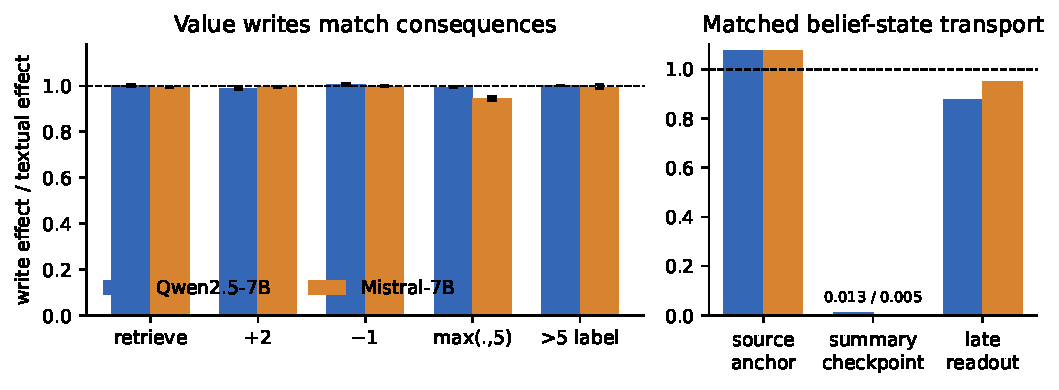
\includegraphics[width=\linewidth]{figures/confirm_effect_matching.pdf}
    \caption{\textbf{Confirmatory effect matching.} Left: early neutral-carrier
    writes reproduce textual-counterfactual effects across direct and computed
    workspace cells in two model families. Right: in the structured-belief
    world, the source-anchor write matches the natural effect while full-state
    transplantation at the designated query-independent checkpoint is nearly
    inert; matched state becomes causally sufficient at the late readout.}
    \label{fig:pilot-effect-matching}
\end{figure}

\subsection{Verbalization redistributes, but does not cleanly relocate, causal load}

Without an explicit verbalized belief, the history-anchor write retains
\PilotVerbalHistoryNoV{} of the natural effect. Adding a contradictory
verbalization reduces the history-only intervention to
\PilotVerbalHistoryV{}, while editing both history and verbalization restores
\PilotVerbalBoth{}. This is consistent with corroborating textual witnesses
rather than a relocation of state, complementing the trained-scratchpad
registers of \citet{shih2026registers}: in stock models, a written statement
appears to join, not replace, the original anchor. A lexical-prior confound
remains, and we report the result as mixed unless the pre-registered
reverse-base control resolves that ambiguity.

\section{What the experiments do and do not establish}

The results support an operational statement: for the tested tasks, source
tokens expose a content- and address-specific write interface whose effects
propagate through downstream computation. The checkpoint intervention is inert
across two model families even though query-specific state becomes causally
sufficient at the late readout. If the grouped probe succeeds, the additional
dissociation will be that the state is linearly readable at a summary position
without that position serving as a causally sufficient register under matched
state transplantation.

This does not imply that state is literally stored in one token, that the model
uses no distributed representation, or that every internal edit follows the
model's natural computation. Autoregressive attention can repeatedly access
the prompt; source-token interventions may alter many later activations. Our
claim concerns causal access and substitutability under specified
interventions.

\section{Limitations}

The tasks use synthetic, tightly controlled prompts and single-token values.
Models are at most 14B parameters and mostly instruction tuned. Quantized
weights are used in several experiments, although residual interventions remain
in floating point. A failed patch is conditional on the tested site, layer,
position, and intervention semantics; it is not proof of representational
absence. Linear probes establish decodability, not use. Finally, many pilot
cells were selected during an exploratory research sequence. We separate those
from the frozen confirmatory battery and will release per-row artifacts so the
distinction is auditable.

\section{Conclusion}

Controlled residual writes provide a way to ask not only what information a
language model represents, but where a bound value can be changed so that its
consequences update coherently. Widened confirmation identifies a reusable
early value write and a sharp causal advantage for source anchors over a
designated summary checkpoint in Qwen and Mistral. The emergence of a strong
late-readout patch effect supplies a matched process control: the intervention
works once query-specific answer state has formed, but not at the earlier
query-independent marker. These findings support token-anchored recomputation
as a concrete mechanism for temporary state in the tested transformer tasks,
while leaving distributed and alternative state representations open.

\bibliographystyle{plainnat}
\bibliography{references}

\appendix
\section{Frozen gates and artifact policy}

The full pre-registration is distributed with the source as
\texttt{PREPRINT\_CONFIRMATORY\_PROTOCOL.md}. Every output stores generated
rows, model identifier, quantization, layer grid, gates, per-row effects, and
random-control summaries. Failed behavioral gates are labeled ineligible.
Discovery pilots and confirmatory artifacts occupy separate directories and
are not pooled.

\end{document}
